% Created 2017-01-14 Sat 10:42
\documentclass[pdf,aspectratio=169]{beamer}
\usepackage[utf8]{inputenc}
\usepackage{graphicx}
\usepackage{longtable}
\usepackage{float}
\usepackage[normalem]{ulem}
\usepackage{hyperref}
\author{Daniel Axtens}
\date{\url{linux.conf.au} 2017 Kernel Miniconf}
\title{Sparse Warnings}
\mode<presentation>{
%\usetheme{Warsaw}
\usetheme{Madrid}
%\usetheme{Berlin}
}
\setcounter{tocdepth}{2}
\begin{document}

\begin{frame}
  \titlepage
\end{frame}

\section{Introduction}
\label{sec-1}

\begin{frame}[c]{Using \texttt{sparse}}
\centering\Large
\texttt{make C=2 ...}
\end{frame}

\begin{frame}{Where we're going}
\tableofcontents
\end{frame}

\section{What does Sparse detect?}
\label{sec-2}

\subsection{Simple things}
\label{sec-2-1}

\begin{frame}[fragile]{Simple static analysis}
\begin{itemize}
\item Undefined/unwise behaviour:
\begin{verbatim}
warning: expression using sizeof bool
warning: odd constant _Bool cast (ffffffffffffffff becomes 1)
\end{verbatim}~\

\item Odd accesses:

\begin{verbatim}
warning: invalid access past the end of 's32' (12 8)
\end{verbatim}
~\

\item Static suggestions:

\begin{verbatim}
warning: symbol 'ppc_fadvise64_64' was not declared. \
Should it be static?
\end{verbatim}

\end{itemize}  
\end{frame}


\subsection{Enhancing \texttt{sparse} with type annotations}
\label{sec-2-2}

\begin{frame}{What does \texttt{sparse} understand?}
\texttt{sparse} + annotations $\Rightarrow$ understanding more than the C compiler alone:
  \begin{itemize}
  \item Endinaness of variables
  \item Address space of pointers
  \item Pointers that should not be dereferenced
  \item Types needing explicit conversion
  \item and (probably) more...
  \end{itemize}
\end{frame}

\subsubsection{Base types}
\label{sec-2-2-1}
\begin{frame}[fragile]{Base types}
\begin{verbatim}
unsigned int instr;
instr = cpu_to_le32(instr);
\end{verbatim}
\pause
\hrule
\begin{verbatim}
warning: incorrect type in assignment (different base types)
   expected unsigned int [unsigned] [assigned] instr
   got restricted __le32 [usertype] <noident>
\end{verbatim}
\end{frame}

\subsubsection{Address spaces}
\label{sec-2-2-2}

\begin{frame}[fragile]{Address spaces}
\begin{verbatim}
unsigned long pc;
int instr;

probe_kernel_address((unsigned int __user *)pc, instr);
\end{verbatim}
\pause
\hrule
\begin{verbatim}
 warning: incorrect type in argument 2 (different address spaces)
    expected void const *src
    got unsigned int [noderef] <asn:1>*<noident>
\end{verbatim}
\end{frame}

\begin{frame}[fragile]{Address spaces}
\begin{verbatim}
struct rt_sigframe __user *frame;

printk_ratelimited(regs->msr & MSR_64BIT ? fmt64 : fmt32,
                   tsk->comm, tsk->pid, "setup_rt_frame",
                   (long)frame, regs->nip, regs->link);
\end{verbatim}
\pause
\hrule
\begin{verbatim}
warning: cast removes address space of expression
\end{verbatim}
\end{frame}

\begin{frame}[fragile]{But wait, there's more!}
\begin{itemize}
\item{no cast types}
{\small
\begin{verbatim}
arch/powerpc/kernel/time.c:361:37: warning: implicit cast to nocast type
arch/powerpc/kernel/time.c:362:29: warning: implicit cast to nocast type
\end{verbatim}}
~\
\item{no dereference pointers (e.g. IO)}
{\small
\begin{verbatim}
arch/powerpc/kernel/io.c:40:24: warning: dereference of noderef expression
arch/powerpc/kernel/io.c:56:18: warning: dereference of noderef expression
\end{verbatim}}
~\
\item{restricted types}
{\small
\begin{verbatim}
arch/powerpc/sysdev/mpic.c:356:18: warning: cast to restricted __le32
\end{verbatim}}
\end{itemize}
\end{frame}

\section{How is Sparse actually used?}
\label{sec-3}

\begin{frame}
\tableofcontents[currentsection]
\end{frame}

\begin{frame}{\#fail}
  \begin{figure}[h!]
    \centering
    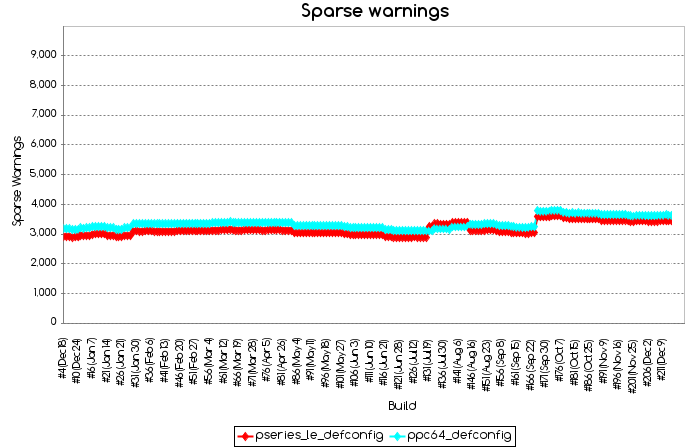
\includegraphics[scale=0.4]{warnings-total-no-spike.png}
    \caption{Sparse warnings, 2 ppc defconfigs, 2016}
    \label{fig:sparse-warnings-no-spike}
  \end{figure}
\end{frame}

\section{Can we improve the situation?}
\label{sec-4}

\begin{frame}
  \tableofcontents[currentsection]
\end{frame}

\subsection{Long term}
\label{sec-4-1}


\begin{frame}{In the long term...}
  Fix the warnings
\end{frame}

\subsubsection{What I've done}
\label{sec-4-1-1}

\begin{frame}{PowerPC warnings}
  \begin{figure}[h!]
    \centering
    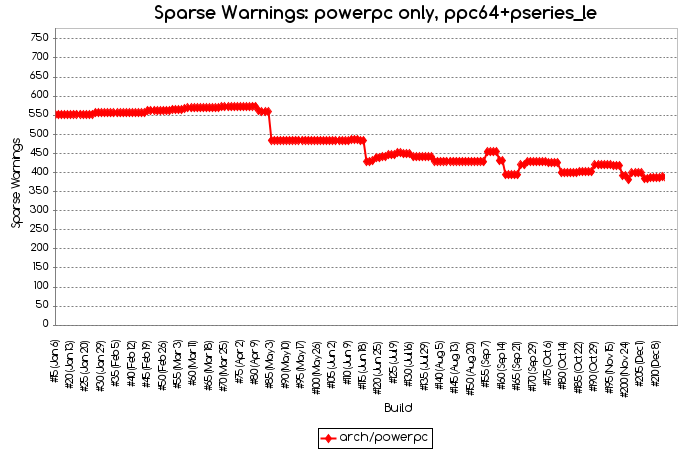
\includegraphics[scale=0.35]{warnings-ppc-no-spike}
    \caption{\texttt{arch/powerpc} sparse warnings, combination of 2 defconfigs, 2016}
    \label{fig:arch-powerpc-warnings-no-spike}
  \end{figure}
\end{frame}

\begin{frame}{PowerPC warnings}
  \begin{figure}[h!]
    \centering
    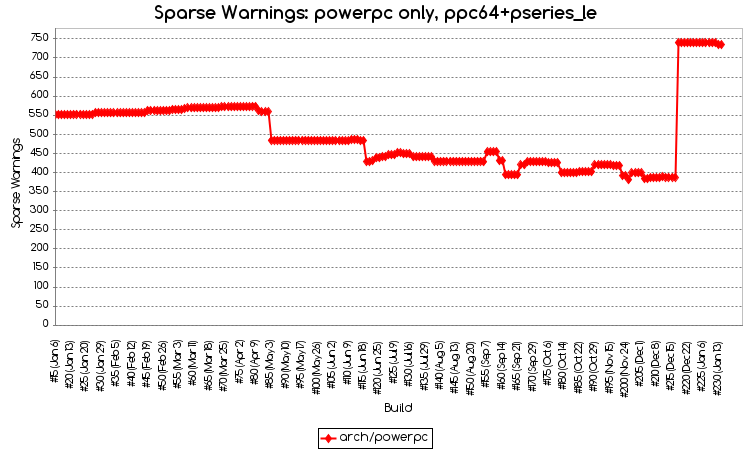
\includegraphics[scale=0.35]{warnings-ppc}
    \caption{\texttt{arch/powerpc} sparse warnings, combination of 2 defconfigs, 2016-present}
    \label{fig:arch-powerpc-warnings-no-spike}
  \end{figure}
\end{frame}

\begin{frame}{Total warnings}
  \begin{figure}[h!]
    \centering
    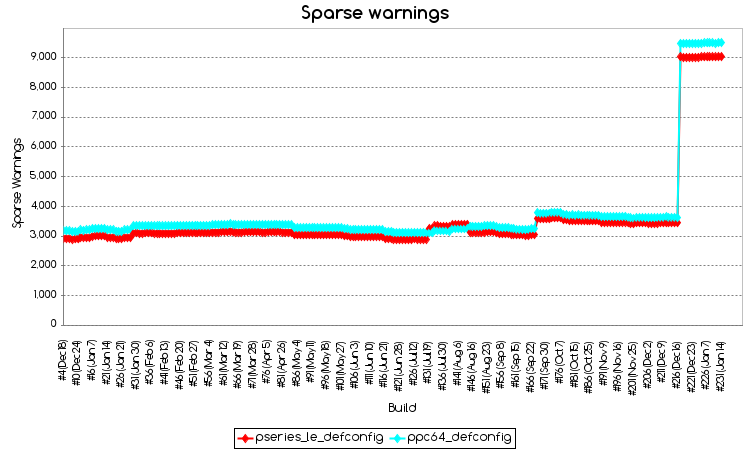
\includegraphics[scale=0.35]{warnings-total.png}
    \caption{Sparse warnings, 2 ppc defconfigs, 2016-present}
    \label{fig:sparse-warnings-no-spike}
  \end{figure}
\end{frame}

\begin{frame}[fragile]{What went wrong? {\small\url{https://patchwork.kernel.org/patch/9467371/}}}
%\footnotesize
    \textbf{\textsc{linux/types.h: enable endian checks for all sparse builds}}
\begin{verbatim}    
    By now, linux is mostly endian-clean. Enabling endian-ness
    checks for everyone produces about 200 new sparse warnings for me -
    less than 10% over the 2000 sparse warnings already there.
    
    Not a big deal, OTOH enabling this helps people notice
    they are introducing new bugs.
    
    So let's just drop __CHECK_ENDIAN__. Follow-up patches
    can drop distinction between __bitwise and __bitwise__.
    
    Cc: Linus Torvalds <torvalds@linux-foundation.org>
    Suggested-by: Christoph Hellwig <hch@infradead.org>
    Signed-off-by: Michael S. Tsirkin <mst@redhat.com>
\end{verbatim}
\end{frame}

\begin{frame}[fragile]{\verb~diff <before> <after>~}
\small
\begin{verbatim}
arch/powerpc/kernel/nvram_64.c:1177:32: warning: cast to restricted __be16

arch/powerpc/kernel/nvram_64.c:893:22: warning: incorrect type in assignment \
    (different base types)
    expected unsigned short [unsigned] [addressable] length 
    got restricted __be16 [usertype] <noident>

arch/powerpc/kvm/book3s_64_vio_hv.c:282:37: warning: cast to restricted __be64

arch/powerpc/kvm/book3s_hv_builtin.c:421:22: warning: incorrect type in assignment \
    (different base types) 
    expected restricted __be32 [addressable] [usertype] xirr 
    got unsigned int

arch/powerpc/perf/hv-24x7.c:1166:18: warning: cast to restricted __be64
\end{verbatim}
\end{frame}
\begin{frame}{In the long term...}
  Fix the warnings
\end{frame}

\subsection{Short term}
\label{sec-4-2}

\begin{frame}{In the short term...}

\textbf{How do you diff compiler warnings/sparse output?}

\begin{itemize}
\item \verb~grep 'arch/powerpc' sparse-output | wc -l~
  \begin{itemize}
  \item Simple, low fidelity.
  \end{itemize}
\item \verb~diff sparse-output-1 sparse-output-2~
  \begin{itemize}
  \item Reordering due to parallel builds
  \item Changing line numbers
  \end{itemize}

\item Write our own.
\end{itemize}
\end{frame}

\begin{frame}{Introducing \texttt{smart-sparse-diff}}
  \url{https://github.com/daxtens/smart-sparse-diff}
\end{frame}
\subsubsection{Demo}
\label{sec-4-3}

\section{Where to from here}
\label{sec-5}
\begin{frame}{Where to from here}
\begin{itemize}
\item \textbf{Fix sparse warnings in your code}
\item When they have reached an acceptably low quantity
\begin{itemize}
\item Contributors: don't add warnings
\item Maintainers: require it of contributors
\item ML reviewers: evaluate it in your reviews
\end{itemize}
\end{itemize}
\end{frame}

\subsection{Sparse as a gateway to kernel development}
\label{sec-5-1}

\begin{frame}{Sparse as a gateway to kernel development}

\begin{itemize}
\item Pick a file with sparse warnings
\item How do patches go into that file?
  \begin{itemize}
  \item What mailing list?
  \item What subject line format?
  \end{itemize}
\item When doing patches:
\begin{itemize}
\item Don't fix just one of many, fix all of one type
\item Compile (and if appropriate, run) test!
\end{itemize}
\item Consult docs on submitting patches:
  \begin{itemize}
  \item Commit messages
  \item How to send a non-broken email
  \end{itemize}
\item Expect bike-shedding.
\end{itemize}

\end{frame}

\section{Conclusion}
\label{sec-6}

\begin{frame}{Conclusion}
\tableofcontents
\end{frame}

\begin{frame}{Legal}
  \begin{itemize}
  \item This work represents the view of the author and does not necessarily represent the view of IBM.
  \item IBM is a registered trademark of International Business Machines Corporation in the United States and/or other countries.
  \item Linux is a registered trademark of Linus Torvalds.
  %\item Microsoft and Windows are trademarks of Microsoft Corporation in the United States, other countries, or both.
  \item Other company, product, and service names may be trademarks or service marks of others.
  \end{itemize}
\end{frame}

\end{document}